\chapter{Numerical experiments} \label{chap:numerical-experiments}

% ~~~~~~~~~~~~~~~~~~~~~~~~~~~~~~~~~~~~~~~~~~~~~~~~~~~~~~~~~~~~~~~~~~~~~~~~~~~~~~~~~~~~~~~~~~~~~~~~~~~~~~~~~~~
\section{Setup} \label{sec:numerical-experiments/setup}

In this section, we present benchmark instances used for evaluating the proposed methods and algorithms,
we describe the modification process for creating problem instances suited to our studied problem,
explain how we obtain (near) optimal solutions to the modeled problem using a constraint programming solver,
and discuss algorithms' parameters used in the following experiments.

All processing, including manipulating with problem instances, solving constraint programming models,
and conducting experiments, all described in the following sections, was done in Python using a library
developed specifically for the purposes of this thesis.
More about the library and running the experiments can be found in \cref{sec:attachments/documentation}.

% -----------------------------------------------------------------------------------------------------------
\subsection{Problem instances} \label{subsec:numerical-experiments/setup/instances}

\citet{Kolisch1997} created the PSPLIB%
\footnote{Available online at \url{https://www.om-db.wi.tum.de/psplib/}}
--- set of benchmark instances for the \ac{rcpsp}.
This set has since been used to evaluate and compare many results in the literature.
(For example, some recent papers from \citet{Bianco2011}, \citet{Cheng2015}, or \citet{Elsayed2017}.)

We will use and modify specific instances from the PSPLIB single-mode instance set.
Instances from this set model the standard \ac{rcpsp}.
They consist of 30, 60, 90, or 120 jobs,
and 4 renewable resources with fixed capacities.
Each job has an execution duration and consumption requirements for each of the resources defined.
Precedences between jobs are stated, forming a single-component precedence graph.
The goal when scheduling such problem instances is usually minimizing the project makespan,
or minimizing the project tardiness with respect to a specified project due date.

To accurately model our studied problem, we introduce several modifications to the original instances.
Namely, we split the precedence graph to create individual order components,
introduce job deadlines, and introduce time-variable resource capacities.
Additionally, to ensure feasibility when modeling specific production systems,
we scale down job durations and resource consumptions.
Following are the modification steps in more detail.

Initially, to model a system with fewer than the original four resources,
we remove the unwanted resources from the problem instance
and optionally adjust the resource consumptions of jobs.
If removing all resources consumed by a job results in that job having no consumption requirements,
the total removed consumption of that job is distributed among the remaining resources.
We then proceed with modifications common for all instances.

First, we split the single-component precedence graph into disconnected components,
creating an inforest.
We do this by ordering the jobs topologically
and selecting one of the last topological generations as seed jobs%
\footnote{The depth of the selected generation influences the number of created components
and the overall structure of the created intree forest.}.
Incrementally, starting with the preceding generation
and continuing in the reverse order of topological generations,
each job from preceding generations selects a single successor precedence
to connect to a successor job.
Analogously, each job from succeeding generations selects a single predecessor precedence
to connect to a predecessor job.
After splitting the graph into an inforest,
the sink-roots of the intrees are selected as orders $\Orders$.

Second, we limit the resource availabilities to simulate working shifts.
The capacity function of a resource is a combination of periodical shift availability
and capacity changes introduced later, in the form of capacity additions and migrations.
We use periodical availability intervals, sub-intervals of $\intinterval{1}{24}$,
to denote that a resource is available each day during the specified time intervals.
During those intervals, the resource capacity is set to its defined shift capacity $\shiftcapacity{k}$;
outside those intervals, the capacity is set to $0$.

Third, we introduce job deadlines.
As stated in \cref{sec:problem-statement/scheduling,sec:problem-statement/constraint-programming-model},
it is sufficient to set deadlines for order jobs $j \in \Orders$ only.
Those were set manually to simulate a continuous distribution of orders in time
as they would appear in a real order-based manufacturing system.

Finally, if needed, the durations of jobs are scaled down appropriately.
Previous modifications might have caused the problem instance to be infeasible
--- a solution to the problem instance could no longer be found.
Such infeasibility can be introduced by limiting resource availabilities to shifts
where the shifts of two resources consumed by a job do not overlap
or overlap for a time duration smaller than the required execution duration of the job.
In such cases, the durations of jobs are scaled down appropriately.
Given that preemption is not allowed and job resource consumptions have to be concurrent,
the maximal duration $\duration{\max}$ of a job in a problem instance is set
to be the length of maximal overlap of all the resources' availabilities in the problem instance.
Then, the durations of all jobs are scaled down as follows:
$$
\duration{j} \gets \frac{\duration{j} \cdot \duration{\max}}%
                        {\max\{\duration{j} \;|\; j \in \Jobs \}}.
$$

We propose 8 problem instance groups, each consisting of 5 individual instances.
The premise is that instances within each group will share similar properties
and that we will be able to analyze aggregated results of evaluations on each group
and draw reasonable conclusions from those results.
\cref{tab:instances} contains an overview of the problem instance groups.
PSPLIB basefile instances were generated using diverse parameter settings,
each setting combined with various random seeds yielding a 10-instance batch.
Each of our instance groups is based on 5 instances from some PSPLIB 10-instance batch,
The specific 5 instances were chosen based on similar precedence graphs
that were formed by the precedence graph-splitting process described above.

\begin{table}[p]
    \centering
    \begin{tabularx}{0.88\textwidth}{lXcX}
        \toprule
        \textbf{Instances} & \textbf{Basefiles} & $|\Resources|$ & \textbf{Resource shifts} \\
        \midrule
        instance01* & j3011\_4.sm, j3011\_2.sm, j3011\_5.sm, j3011\_6.sm, j3011\_9.sm
                    & 4 
                    & R1: M $|$ A $|$  \newline
                      R2: M $|$ A $|$  \newline
                      R3: M $|$ A $|$  \newline
                      R4: M $|$ A $|$
                    \\
                    \cmidrule[0.01em](lr){1-4}
        instance02* & j3010\_2.sm, j3010\_4.sm, j3010\_5.sm, j3010\_7.sm, j3010\_8.sm
                    & 2 
                    & R1: M $|$ A $|$ N \newline
                      R2: M $|$ A $|$
                    \\
                    \cmidrule[0.01em](lr){1-4}
        instance03* & j6010\_7.sm, j6010\_8.sm, j6010\_9.sm, j6010\_6.sm, j6010\_2.sm 
                    & 1 
                    & R1: M $|$ A $|$ 
                    \\
                    \cmidrule[0.01em](lr){1-4}
        instance04* & j6010\_7.sm, j6010\_8.sm, j6010\_9.sm, j6010\_6.sm, j6010\_2.sm
                    & 1 
                    & R1: M $|$ A $|$
                    \\
                    \cmidrule[0.01em](lr){1-4}
        instance05* & j6011\_10.sm, j6011\_2.sm, j6011\_3.sm, j6011\_6.sm, j6011\_7.sm
                    & 4 
                    & R1: M $|$ A $|$ \newline
                      R2: M $|$ A $|$ \newline
                      R3: \phantom{M} $|$ A $|$ N \newline
                      R4: M $|$ A $|$ N
                    \\
                    \cmidrule[0.01em](lr){1-4}
        instance06* & j6013\_6.sm, j6013\_2.sm, j6013\_3.sm, j6013\_5.sm, j6013\_10.sm
                    & 4 
                    & R1: \phantom{M} $|$ A $|$ \newline
                      R2: \phantom{M} $|$ A $|$ \newline
                      R3: \phantom{M} $|$ A $|$ \newline
                      R4: \phantom{M} $|$ A $|$
                    \\
                    \cmidrule[0.01em](lr){1-4}
        instance07* & j1201\_1.sm, j1201\_3.sm, j1201\_6.sm, j1201\_7.sm, j1201\_10.sm
                    & 4 
                    & R1: M $|$ A $|$ \newline
                      R2: M $|$ A $|$ \newline
                      R3: M $|$ A $|$ \newline
                      R4: M $|$ A $|$
                    \\
                    \cmidrule[0.01em](lr){1-4}
        instance08* & j1205\_1.sm, j1205\_5.sm, j1205\_6.sm, j1205\_7.sm, j1205\_9.sm
                    & 2 
                    & R1: M $|$ A $|$ \newline
                      R2: M $|$ A $|$
                    \\
        \bottomrule
    \end{tabularx}
    \caption{
        Overview of the experiment instances used.
        For each instance group,
        the "Basefiles" column contains names of the PSPLIB instances
        used to create the five instances from the group.
        Following are columns describing the resource characteristics of the instance group ---
        the number of resources and the resource availability profiles.
        The resource availability profiles consist of three possible shifts ---
        morning (M), afternoon (A), and night (N) ---
        representing that the resource is available each day (period of 24 time periods)
        during the corresponding multiples of the time periods
        $\intinterval{7}{14}$, $\intinterval{15}{22}$, and $\intinterval{1}{6} \cup \{23, 24\}$ respectively.
        }
    \label{tab:instances}
\end{table}

% -----------------------------------------------------------------------------------------------------------
\subsection{Solving the constraint programming model} \label{subsec:numerical-experiments/setup/solving-cp-model}

We use the \ac{docplex}%
\footnote{See online at \url{https://ibmdecisionoptimization.github.io/docplex-doc/cp/index.html}.}
Python API for modeling the problems via constraint programming.
We then utilize the \ac{cpopt}%
\footnote{See online at \url{https://www.ibm.com/products/ilog-cplex-optimization-studio/cplex-cp-optimizer}. \citep{WEB_IBM_CPLEX}}
for finding optimal solutions to the modeled problems.

Solver time limit was set to 10 seconds.
Upon reaching the time limit without optimality verification,
the best solution found so far was used.
This follows from the argument that for the proposed methods
to be applicable in real-world manufacturing systems,
they need to be reasonably fast
--- not much time can be spent finding optimal solutions to the problem instances\footnote{
    Such an argument could lead to the preference of heuristic approaches for finding problem instance solutions.
    However, as discussed in \cref{subsec:related-works/scheduling-the-rcpsp/solution-approaches},
    the benefits of utilizing an exact constraint programming solver outweigh the herein-mentioned drawbacks.
    }.

We use solver hot-starting to speed up consecutive solution finding of modified problem instances.
Models of modified instances usually differ only slightly from the models of the original problem instance.
This means, that an (optimal) solution to the original problem instance
might remain a feasible (if not directly an optimal) solution to a modified version of the problem instance.
If not, it is still probable that the desired feasible solution to the modified problem instance
does not differ much from the initial solution to the original problem instance.

Hot-starting of the constraint programming solver utilizes this
by starting the search not from a random initial solution, but from a particular given solution.
With high probability, a feasible solution will be found shortly
which consequently speeds up the process of finding an optimal one.
In summary, consecutively finding solutions to modified problem instances will usually be faster
than finding the initial solution to the original problem instance.

% -----------------------------------------------------------------------------------------------------------
\subsection{Algorithm parameters} \label{subsec:numerical-experiments/setup/algorithm-parameters}

For both evaluated algorithms, we choose multiple different combinations of parameters.
Then, on each problem instance, the algorithms are evaluated using every parameter combination.
As a result, for each instance and for each algorithm we will have a set of evaluations,
each evaluation corresponding to a specific parameter combination.
The parameters of the algorithms will be constructed from all possible combinations
of the following parameter values, separate for each algorithm.
\begin{enumerate}[label=(\roman*)]
    \item \emph{\acl{iira}}
        \begin{itemize}
            \item Bottleneck identification indicator $\algIndicator \in \{ \indMRUR{}, \indAUAU{} \}$
            \item Granular period granularity $\algGranularity \in \{ 4, 8 \}$
            \item Improvement potential convolution kernel $\algConvolution \in \{ \convPre, \convAround, \convPost \}$
            \item Number of iterations $\algMaxiter \in \{ 1, 2, 3 \}$
            \item Number of improvement periods $\algMaxperiods \in \{ 1, 2, 3, 4 \}$
            \item Capacity improvement $\algImprovement \in \{ 4, 10 \}$
        \end{itemize}

    \item {\emph{\acl{ssira}}}
        \begin{itemize}
            \item Interval sort key $\algSortkey \in \{ \algSortkeyTime, \algSortkeyImprovement \}$
            \item Number of iterations $\algMaxiter \in \{ 1, 2, 3 \}$
            \item Number of improvement intervals $\algMaxintervals \in \{ 1, 2, 3, 4, 5, 6 \}$
        \end{itemize}
\end{enumerate}

Regarding the possible improvement potential convolution kernels of the \ac{iira},
see diagrams of the kernels in \cref{fig:convolutions}.
Regarding the \ac{ssira} and its possible interval sort keys,
the $\algSortkeyTime$ is a sort key which orders the improvement intervals
by the time periods during which the intervals are proposed in a descending order.
Using this key, improvement intervals identified later in the schedule
precede improvement intervals identified earlier in the schedule.
The $\algSortkeyImprovement$ orders the improvement intervals
by the improvement in job start times they represent.
Using this key, improvement intervals proposing large improvements of job start times
precede improvement intervals which propose smaller improvements of job start times.

\begin{figure}[hbt]
    \centering
    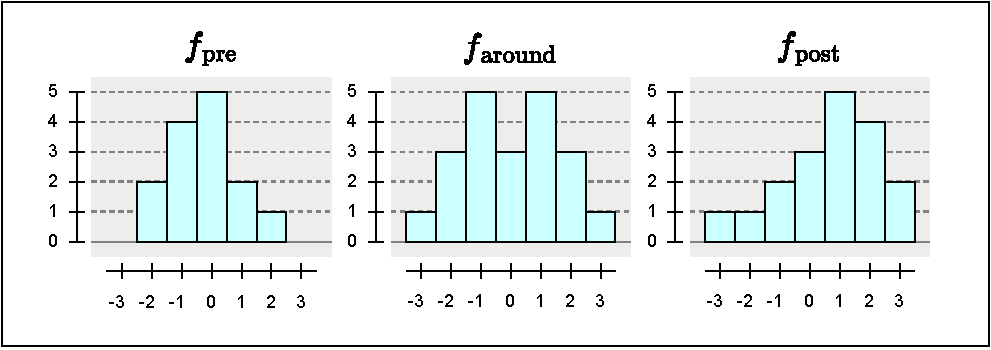
\includegraphics[width=\textwidth]{img/Convolutions.pdf}
    \caption{Improvement convolution kernels used in the \ac{iira} algorithm.}
    \label{fig:convolutions}
\end{figure}

The parameter value ranges were set based on prior testing of the algorithms.
We do not deny the possibility that a promising combination of parameters
with great performance potential was not included in the constructed set of combinations,
nor do we claim those ranges are exhaustive in terms of acceptable values.
The value ranges were set to create a broad spectrum of algorithms with comparable performances.

When considering the number of iterations for example,
the maximum value was set reasonably low as both algorithms
tend to propose impractical relaxations after several iterations.
For example, the algorithms would propose to disregard any planned resource working shift pauses
or double the resource capacities throughout most of the scheduling horizon.
While such proposals would certainly achieve the desired improvement,
they are not realistic within the context of real-world manufacturing systems.

The combinations of all algorithm parameters
for the \ac{iira} form a total of 288 different parameter combinations and
for the \ac{ssira} a total of 36 different parameter combinations.
We justify this apparent difference in the parameter combinations totals
simply by the fact that the \ac{iira} is an algorithm with more parameters by design.
To sufficiently evaluate the \ac{iira}, we provide several values for each parameter.
Reducing the choices would leave out interesting combinations of parameters.
Conversely, additional value options for the parameters of the \ac{ssira}
would not introduce any more interesting combinations.
We did not come up with other improvement interval sorting keys which would seem practical
and we already discussed the impracticality of a larger number of algorithm iterations.

% ---------------------------------------------------------------
\subsection{Methods of evaluation} \label{subsec:numerical-experiments/setup/methods-of-evaluation}

To evaluate an algorithm, we follow the procedure stated in \cref{sec:problem-statement/relaxed-schedule}.
We start with a given problem instance $\Instance$ for which we obtain a solution $\Schedule$.
Then, we run the algorithm with specified parameters,
the output of which is the modified instance $\Instance^*$ and its solution $\Schedule^*$.
Finally, we compute the following metrics:
\begin{itemize}
    \item
        Tardiness improvement
        $$
        \kpiImprovement \defeq \tardiness{o} - \tardiness{o}^*.
        $$
        This metric is arguably the most important, as it tells us how much the algorithm was able
        to reduce the tardiness of the target order $\targetOrder$.
    
    \item
        Solution difference
        $$
        \kpiDiff \defeq \sum_{j \in J} \abs{\jobend{j} - \jobend{j}^*}.
        $$
        This metric shows how much the modified solution differs from the original solution.
        It hints about how challenging it would be to realize the proposed modifications.
        For instance, in manufacturing setups that employ human workers,
        working shifts may be planned weeks in advance.
        Therefore, significant changes to the work plan for the upcoming days
        may not be feasible.

    \item
        Instance modification cost
        $$
        \kpiCost \defeq
            \costAddition \left(
                \sum_{\addition{k}{s}{e}{c} \in \Additions^{\Instance^*}} (e - c) c
            \right)
            +
            \costMigration \left(
                \sum_{\migration{k_\text{f}}{k_\text{t}}{s}{e}{c} \in \Migrations^{\Instance^*}} (e - c) c
            \right),
        $$
        where $\costAddition$ is a given capacity addition cost
        and $\costMigration$ is a given capacity migration cost.

    \item 
        We also measure the algorithm computation time, denoted as $\kpiDuration$,
        which is the total run-time of the evaluated algorithm in seconds.
        This computation time will mostly consist of finding solutions to modified problems ---
        the computation time of the \ac{cpopt}.
\end{itemize}

% ~~~~~~~~~~~~~~~~~~~~~~~~~~~~~~~~~~~~~~~~~~~~~~~~~~~~~~~~~~~~~~~~~~~~~~~~~~~~~~~~~~~~~~~~~~~~~~~~~~~~~~~~~~~
\section{Comparative results} \label{sec:numerical-experiments/comparative-results}

In this section, we present the experiment results.
All experiments were conducted on a personal desktop computer equipped with an 
Intel\textsuperscript{\textregistered}~Core\texttrademark\ i5-8400~CPU and 16~GB of RAM.

The total evaluation time was 43 hours, 5 minutes, and 40 seconds.
This time is the sum of the individual durations of each algorithm evaluation.
As described in \cref{subsec:numerical-experiments/setup/methods-of-evaluation},
the measured time does not include the experiment running overhead nor aggregate data manipulation,
but such overheads are negligible in comparison to the experiment evaluation times.

Plots in this section, namely \cref{fig:exp/cost-improv,fig:exp/improv-diff,fig:exp/duration-improv},
present the evaluation results split into 4 sets.
We choose the arguably most important parameters for each of the algorithms,
the bottleneck identification indicator for the \ac{iira}
and the improvement interval sort key for the \ac{ssira},
for splitting the sets of evaluations to present how performances of the algorithms differ
based on the choice of those parameters.
For the \ac{iira},
we split the evaluations by the bottleneck resource identification indicator parameter $\algIndicator$,
yielding two sets of evaluations
for each of the two employed adapted identification indicators \ac{mrur} and \ac{auau}.
For the \ac{ssira},
we split the evaluations by the sort key parameter $\algSortkey$,
yielding two sets of evaluations for each of the two choices of the sort key parameter
$\algSortkeyTime$ and $\algSortkeyImprovement$.

We could further split the larger parameter sets for the \ac{iira}
by the improvement potential convolution kernel parameter
as this parameter also has a considerable influence on the algorithm functioning.
However, such split would create 6 evaluation sets for the \ac{iira}.
Plotting results for this many different evaluation sets
would negate the advantages of splitting the evaluations.

% -----------------------------------------------------------------------------------------------------------
\subsection{Observations}

\Cref{tab:exp/improvements} provides a summary of achieved improvements on the individual instance groups.
The \ac{iira} found improvements for $72.5\%$ of the instances,
while the \ac{ssira} found improvements for $87.5\%$ of the instances.
The \ac{iira} found a better improvement than the \ac{ssira} on $10$ instances.
Conversely, the \ac{ssira} found a better improvement than the \ac{iira} on $13$ instances,
and on $6$ of these, the \ac{ssira} was the only algorithm to find an improvement.
There were no instances where the \ac{iira} found an improvement and the \ac{ssira} did not.
Where it found an improvement, the \ac{iira} found a solution
with the overall best improvement for $75.8\%$ of the instances,
while the \ac{ssira} did so for $71.4\%$ of the instances.

\begin{table}[bt]
    \centering
    \pgfplotstabletypeset[
        header=true, % Data file contains header
        columns={Instances,{IIRA improved},{IIRA improved unique},{IIRA improved best},{SSIRA improved},{SSIRA improved unique},{SSIRA improved best}},
        col sep=tab, % Set the column separator to tab
        every head row/.style={
            before row={
            \toprule
            & \multicolumn{3}{c}{\acs{iira}} & \multicolumn{3}{c}{\acs{ssira}} \\
            },
            after row=\midrule,
            },
        every last row/.style={
            before row={\midrule},
            after row={\bottomrule},
            },
        columns/Instances/.style={
            string type,
            string replace*={_}{\_},
            column type=l,
            },
        columns/IIRA improved/.style={
            column name={Improved},
            column type=c,
            string type,
            },
        columns/IIRA improved unique/.style={
            column name={Unique},
            column type=c,
            string type,
            },
        columns/IIRA improved best/.style={
            column name={Best},
            column type=c,
            string type,
            },
        columns/SSIRA improved/.style={
            column name={Improved},
            column type=c,
            string type,
            },
        columns/SSIRA improved unique/.style={
            column name={Unique},
            column type=c,
            string type,
            },
        columns/SSIRA improved best/.style={
            column name={Best},
            column type=c,
            string type,
            },
    ]{tables/data_instances.tsv}
    \caption{
        Number of improved solutions found in the instance groups.
        For each algorithm, the first column contains the number of instances
        within the specified instance group for which an improved solution was found
        The second column contains the number of instances for which an improved solution was found
        and for which the other algorithm did not find an improvement
        The third column contains the number of instances for which the solution
        with best improvement was found by this algorithm.
        }
    \label{tab:exp/improvements}
\end{table}



\Cref{tab:exp/kpis-improvements} contains results concerning the achieved tardiness improvements.
Instances for which no algorithm found any improvements were omitted.
For each instance, the table lists
the average cost per unit tardiness improvement (per time period)
and the average tardiness improvement achieved per unit of evaluation time (per second).
Out of the 29 instances where both algorithms found improving solutions,
the \ac{iira} had a lower average cost per unit tardiness improvement on 15 of them.
The \ac{iira} algorithm achieved a better average on all the instances
within the instance group \instGroup{8}, except for \inst{8}{4},
where the only improvement was found by the \ac{ssira}.
No clear trend is observed in the average cost per unit tardiness improvement apart from this group.

Regarding the average improvement achieved per unit of evaluation time,
the \ac{iira} algorithm performed slightly better than the \ac{ssira} algorithm.
Out of the 29 instances improved by both,
the \ac{iira} achieved a greater improvement per unit time on 18 instances.
This pattern is particularly evident on the instance groups
\instGroup{3}, \instGroup{5}, and \instGroup{7}.

\input{chapters/4a-results} % TABLES AND PLOTS ~~~~~~~~~~~~~~~~~~~~~~~~~~~~~~~~~~~~~~~~~~~~~~~~~~~~~~~~~~~~~~
\begin{table}[p]
    \centering
    \pgfplotstabletypeset[
        header=true, % Data file contains header
        columns={Instance,{IIRA avg cost per improvement},{IIRA avg improvement per duration},{SSIRA avg cost per improvement},{SSIRA avg improvement per duration}},
        col sep=tab, % Set the column separator to tab
        skip rows between index={2}{4},
        skip rows between index={7}{8},
        skip rows between index={28}{30},
        every head row/.style={
            before row={
            \toprule
            & \multicolumn{4}{c}{\acs{iira}} & \multicolumn{4}{c}{\acs{ssira}} \\
            },
            after row=\midrule,
        },
        every row no 2/.style={after row={\midrule}},
        every row no 6/.style={after row={\midrule}},
        every row no 11/.style={after row={\midrule}},
        every row no 16/.style={after row={\midrule}},
        every row no 21/.style={after row={\midrule}},
        every row no 24/.style={after row={\midrule}},
        every row no 29/.style={after row={\midrule}},
        every last row/.style={after row={\bottomrule}},
        columns/Instance/.style={
            string type,
            string replace*={_}{\_},
            column type=l,
            },
        columns/IIRA avg cost per improvement/.style={
            column name=$\mean{\kpiCost / \kpiImprovement}$,
            column type=c,
            fixed, precision=2,
            dec sep align,
            clear infinite,
            },
        columns/IIRA avg improvement per duration/.style={
            column name=$\mean{\kpiImprovement / \kpiDuration}$,
            column type=c,
            fixed, precision=2,
            dec sep align,
            clear infinite,
            },
        columns/SSIRA avg cost per improvement/.style={
            column name=$\mean{\kpiCost/ \kpiImprovement} $,
            column type=c,
            fixed, precision=2,
            dec sep align,
            clear infinite,
            },
        columns/SSIRA avg improvement per duration/.style={
            column name=$\mean{\kpiImprovement / \kpiDuration}$,
            column type=c,
            fixed, precision=2,
            dec sep align,
            clear infinite,
            },
    ]{tables/data_kpis.tsv}
    \caption{
        Results concerning the achieved improvement.
        For each algorithm, the~first column represents the average cost per unit of improvement,
        the~second column represents the average improvement per unit of computation time.
        Instances for which no algorithm found any improvements were omitted.
        }
    \label{tab:exp/kpis-improvements}
\end{table}



\Cref{tab:exp/kpis-difference} contains results concerning induced schedule difference.
Instances for which no algorithm found any improvements were omitted.
For each instance, the table lists
the average schedule difference induced in individual evaluations
and the average difference across jobs within that instance.
On smaller instances, such as in instance groups \instGroup{2}, \instGroup{3}, and \instGroup{4},
the \ac{iira} proposes better solutions that differ from the original schedule
less than those proposed by the \ac{ssira}.
Conversely, on larger instances, such as in instance groups \instGroup{7} or \instGroup{8},
the \ac{iira} proposes solutions with a larger schedule impact than the \ac{ssira}.
We observe, that in terms of schedule difference
the \ac{iira} proposes better solutions on smaller instances while
the \ac{ssira} is more effective on larger instances.
Exceptions exist, for example on the instances \inst{3}{4} or \inst{5}{2},
where the \ac{ssira} proposes significantly less disruptive solutions.
In the evaluations of the \ac{ssira} algorithm on the instance group \instGroup{7},
we observe that while the \ac{iira} has comparable results across all five instances,
the \ac{ssira} performs significantly better on instances \inst{7}{2} and \inst{7}{3}.
A similar anomaly can be observed on the instance \inst{5}{2} within the instance group \instGroup{5}.
Conversely, within the instance group \instGroup{4},
all evaluations of the \ac{ssira} are consistent across the individual instances,
but the performance of the \ac{iira} on instance \inst{4}{2} is notably worse.

\begin{table}[p]
    \centering
    \pgfplotstabletypeset[
        header=true, % Data file contains header
        columns={Instance,{IIRA avg diff},{IIRA avg diff per job},{IIRA avg diff per improvement},{SSIRA avg diff},{SSIRA avg diff per job},{SSIRA avg diff per improvement}},
        col sep=tab, % Set the column separator to tab
        skip rows between index={2}{4},
        skip rows between index={7}{8},
        skip rows between index={28}{30},
        every head row/.style={
            before row={
            \toprule
            & \multicolumn{6}{c}{\acs{iira}} & \multicolumn{6}{c}{\acs{ssira}} \\
            },
            after row=\midrule,
        },
        every row no 2/.style={after row={\midrule}},
        every row no 6/.style={after row={\midrule}},
        every row no 11/.style={after row={\midrule}},
        every row no 16/.style={after row={\midrule}},
        every row no 21/.style={after row={\midrule}},
        every row no 24/.style={after row={\midrule}},
        every row no 29/.style={after row={\midrule}},
        every last row/.style={after row={\bottomrule}},
        columns/Instance/.style={
            string type,
            string replace*={_}{\_},
            column type=l,
            },
        columns/IIRA avg diff/.style={
            column name=$\mean{\kpiDiff}$,
            column type=c,
            fixed, precision=2,
            dec sep align,
            clear infinite,
            },
        columns/IIRA avg diff per job/.style={
            column name=$\mean{\kpiDiff} / n$,
            column type=c,
            fixed, precision=2,
            dec sep align,
            clear infinite,
            },
        columns/IIRA avg diff per improvement/.style={
            column name=$\mean{\kpiDiff / \kpiImprovement}$,
            column type=c,
            fixed, precision=2,
            dec sep align,
            clear infinite,
            },
        columns/SSIRA avg diff/.style={
            column name=$\mean{\kpiDiff}$,
            column type=c,
            fixed, precision=2,
            dec sep align,
            clear infinite,
            },
        columns/SSIRA avg diff per job/.style={
            column name=$\mean{\kpiDiff} / n$,
            column type=c,
            fixed, precision=2,
            dec sep align,
            clear infinite,
            },
        columns/SSIRA avg diff per improvement/.style={
            column name=$\mean{\kpiDiff / \kpiImprovement}$,
            column type=c,
            fixed, precision=2,
            dec sep align,
            clear infinite,
            },
    ]{tables/data_kpis.tsv}
    \caption{
        Results concerning the induced schedule difference.
        For each algorithm, the~first column represents the average schedule difference found for the instance,
        the~second column represents the average difference in start times per job in the instance.
        Instances for which no algorithm found any improvements were omitted.
        }
    \label{tab:exp/kpis-difference}
\end{table}

In \cref{fig:exp/cost-improv} we present the results concerning
capacity changes cost related to tardiness improvement, aggregated over the individual instance groups.
Note that the capacity changes costs (x-axis) are plotted on a logarithmic scale.
We observe a consistent trend for the \ac{ssira} with the $\algSortkeyTime$ sort key:
better improvements can be achieved with increasing costs.
Smaller improvements require smaller costs,
while seeking further improvements requires an increase in costs.
A similar pattern is observed for the \ac{ssira} with the $\algSortkeyImprovement$ sort key;
however, on certain smaller instance groups such as \instGroup{1} or \instGroup{4},
the improvement achieved for the same cost can vary significantly.
An interesting observation is that on smaller instances,
such as in instance groups \instGroup{2}, \instGroup{3}, and \instGroup{4},
the \ac{iira} finds solutions with the same improvement to cost ratio
using both bottleneck identification indicators.
This is not the case on larger instances,
where the evaluations employing the \ac{auau} and \ac{mrur} indicators differ substantially.
An important observation is that, particularly on larger instances,
the \ac{iira} is capable of finding significant improvements with relatively lows costs.
This is apparent on instance groups \instGroup{7} and \instGroup{8},
where the best improvements for given costs are almost exclusively found by the \ac{iira},
whereas the \ac{ssira} only finds minor improvements.

In \cref{fig:exp/improv-diff} we present the results concerning
tardiness improvement related to induced schedule difference, aggregated over the individual instance groups.
We observe a consistent trend for the \ac{ssira} with the $\algSortkeyTime$ sort key:
greater tardiness improvement corresponds with an increased schedule difference.
This trend is also observable for other evaluations.
Evaluations of the \ac{ssira} with the $\algSortkeyImprovement$ sort key are the most inconsistent,
particularly on smaller instances.
In general, the \ac{ssira} utilizing the $\algSortkeyImprovement$ sort key tends to propose
the least favorable solutions in terms of the induced schedule difference.
On larger instances, most evaluations follow the linear increasing trend.
Notably, in instance groups \instGroup{1}, \instGroup{4}, or \instGroup{6},
the \ac{ssira} utilizing the $\algSortkeyTime$ finds solutions with improvement comparable
to those proposed by the \ac{ssira} utilizing the $\algSortkeyImprovement$ sort key
and the \ac{iira},
but with a lower schedule difference.
On larger instances, the \ac{ssira} utilizing the $\algSortkeyTime$ appears to be unable to find
solutions with the overall best improvements.
For the solutions with the highest improvement,
the \ac{iira} proposes marginally better solutions than the \ac{ssira},
if any are found by the \ac{ssira}.

In \cref{fig:exp/duration-improv} we present the results concerning
evaluation computation time related to tardiness improvement, aggregated over the individual instance groups.
These results are notably inconsistent.
We observe that evaluation times of the \ac{ssira} are more varied than those of the \ac{iira}.
This is particularly apparent on the instance groups \instGroup{4}, \instGroup{7}, and \instGroup{8}.
Additionally, we observe that in some cases,
most notably on instances from the instance groups \instGroup{6} and \instGroup{8},
the evaluations form linear clusters with identical evaluation times.

\begin{figure}[p]
    \centering
    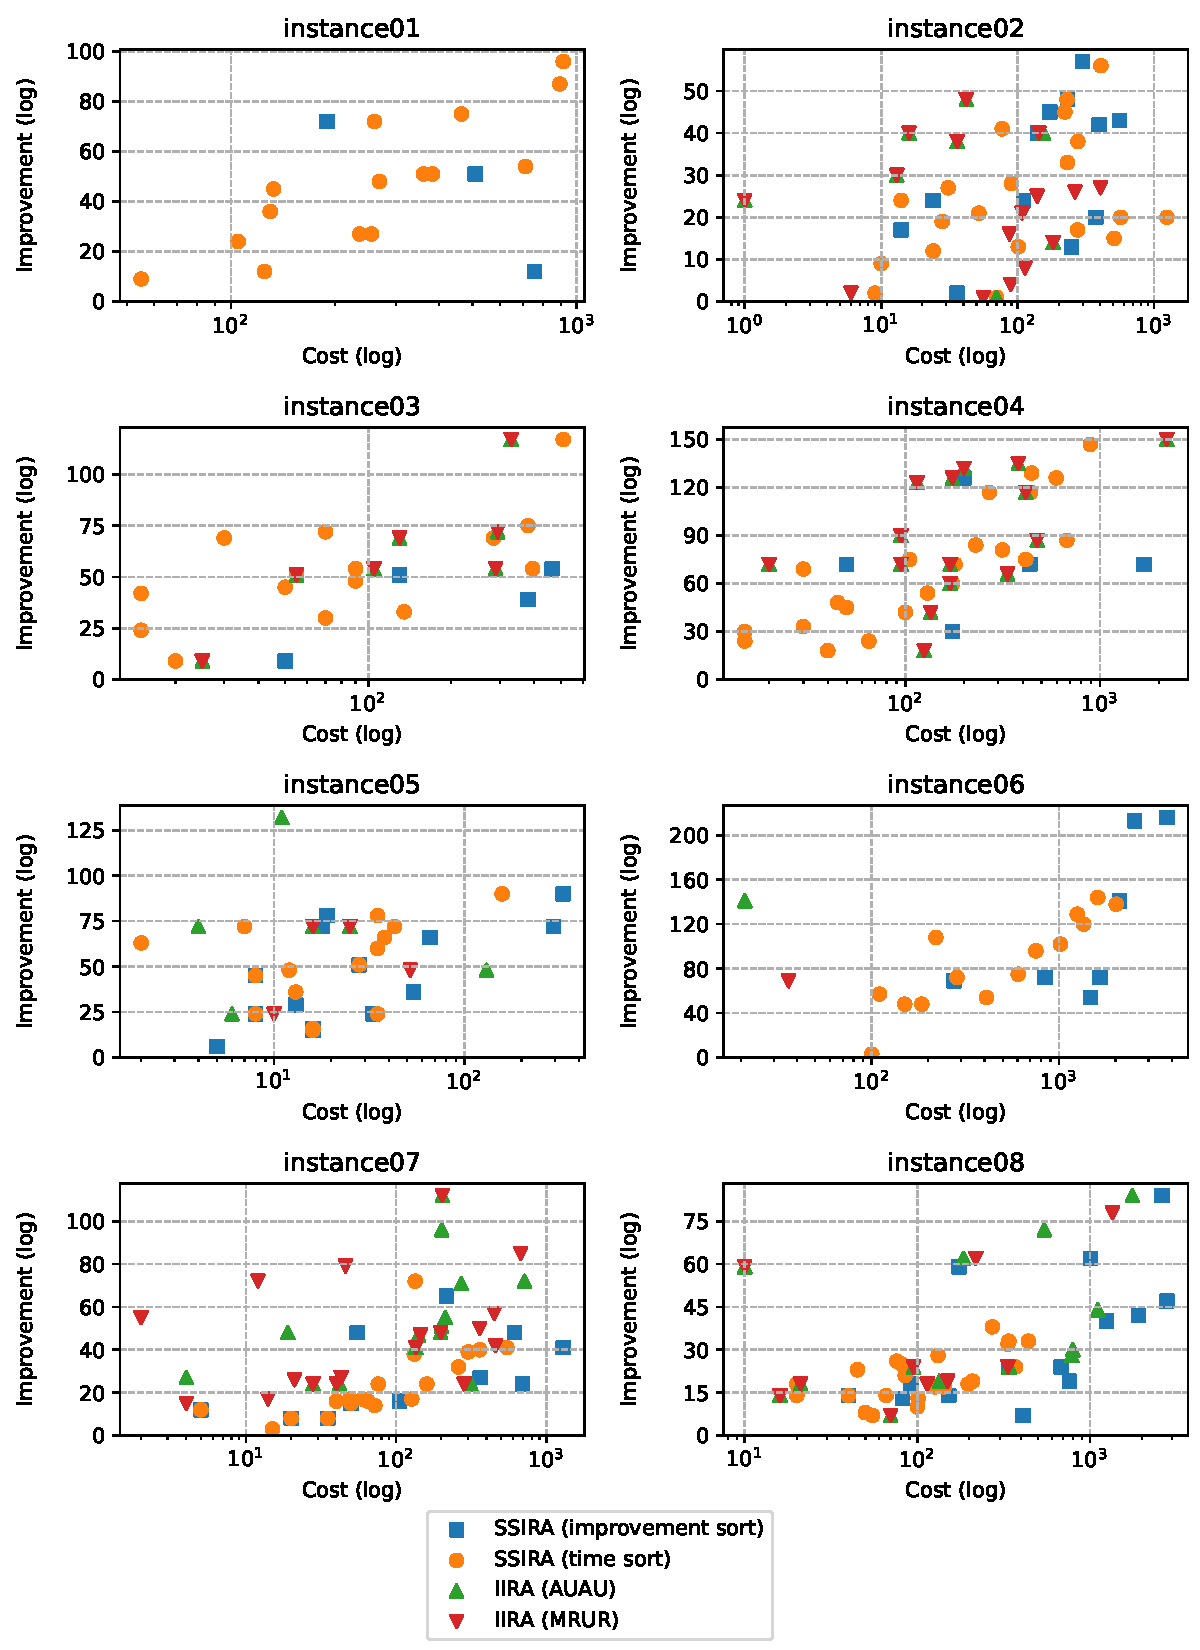
\includegraphics[width=\textwidth]{img/exp_aggregated_cost_improv.pdf}
    \caption{
        Aggregated plots of capacity changes costs (x-axis) to achieved improvement (y-axis).
        In each plot, every algorithm evaluation comprises of five Pareto fronts of evaluations
        on the five individual instances from the represented instance group.
        Full non-aggregated results for each individual instance can be found in \cref{fig:exp-full/cost-improv}.
        }
    \label{fig:exp/cost-improv}
\end{figure}

\begin{figure}[p]
    \centering
    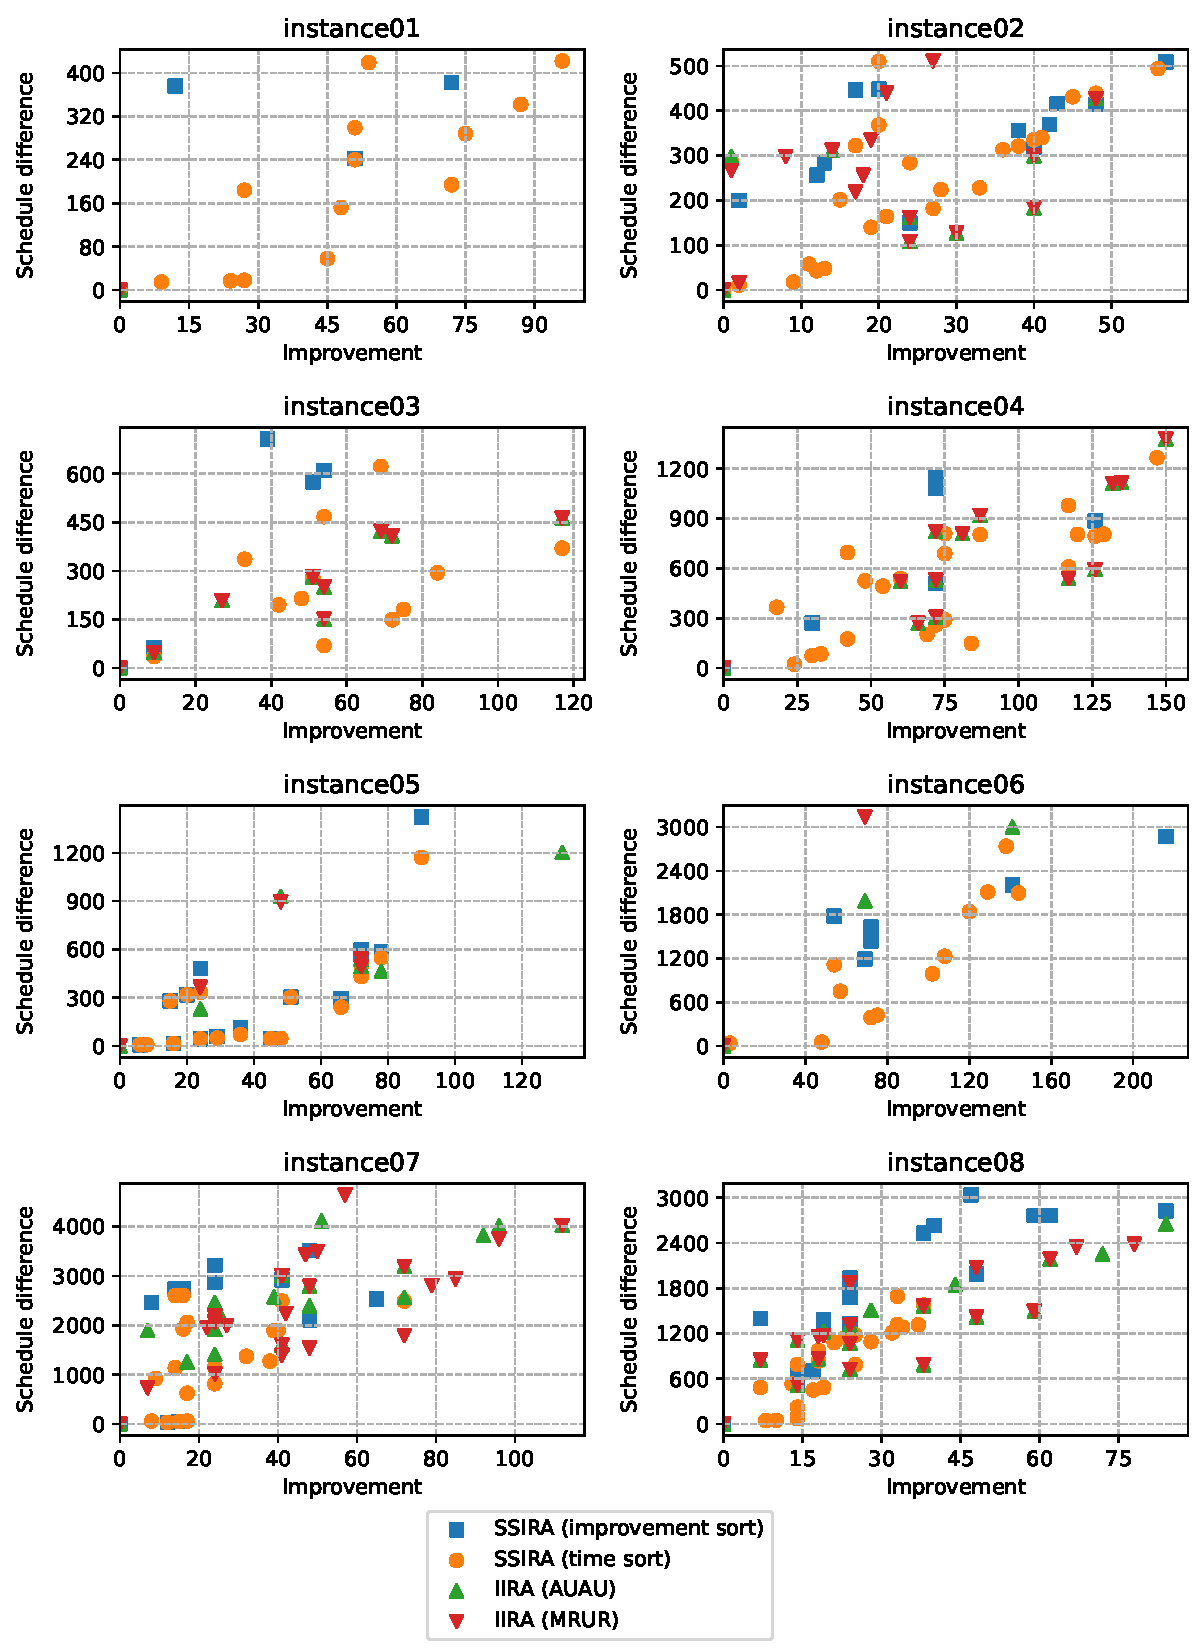
\includegraphics[width=\textwidth]{img/exp_aggregated_improv_diff.pdf}
    \caption{
        Aggregated plots of achieved improvement (x-axis) to induced schedule difference (y-axis).
        In each plot, every algorithm evaluation comprises of five Pareto fronts of evaluations
        on the five individual instances from the represented instance group.
        Full non-aggregated results for each individual instance can be found in \cref{fig:exp-full/improv-diff}.
        }
    \label{fig:exp/improv-diff}
\end{figure}

\begin{figure}[p]
    \centering
    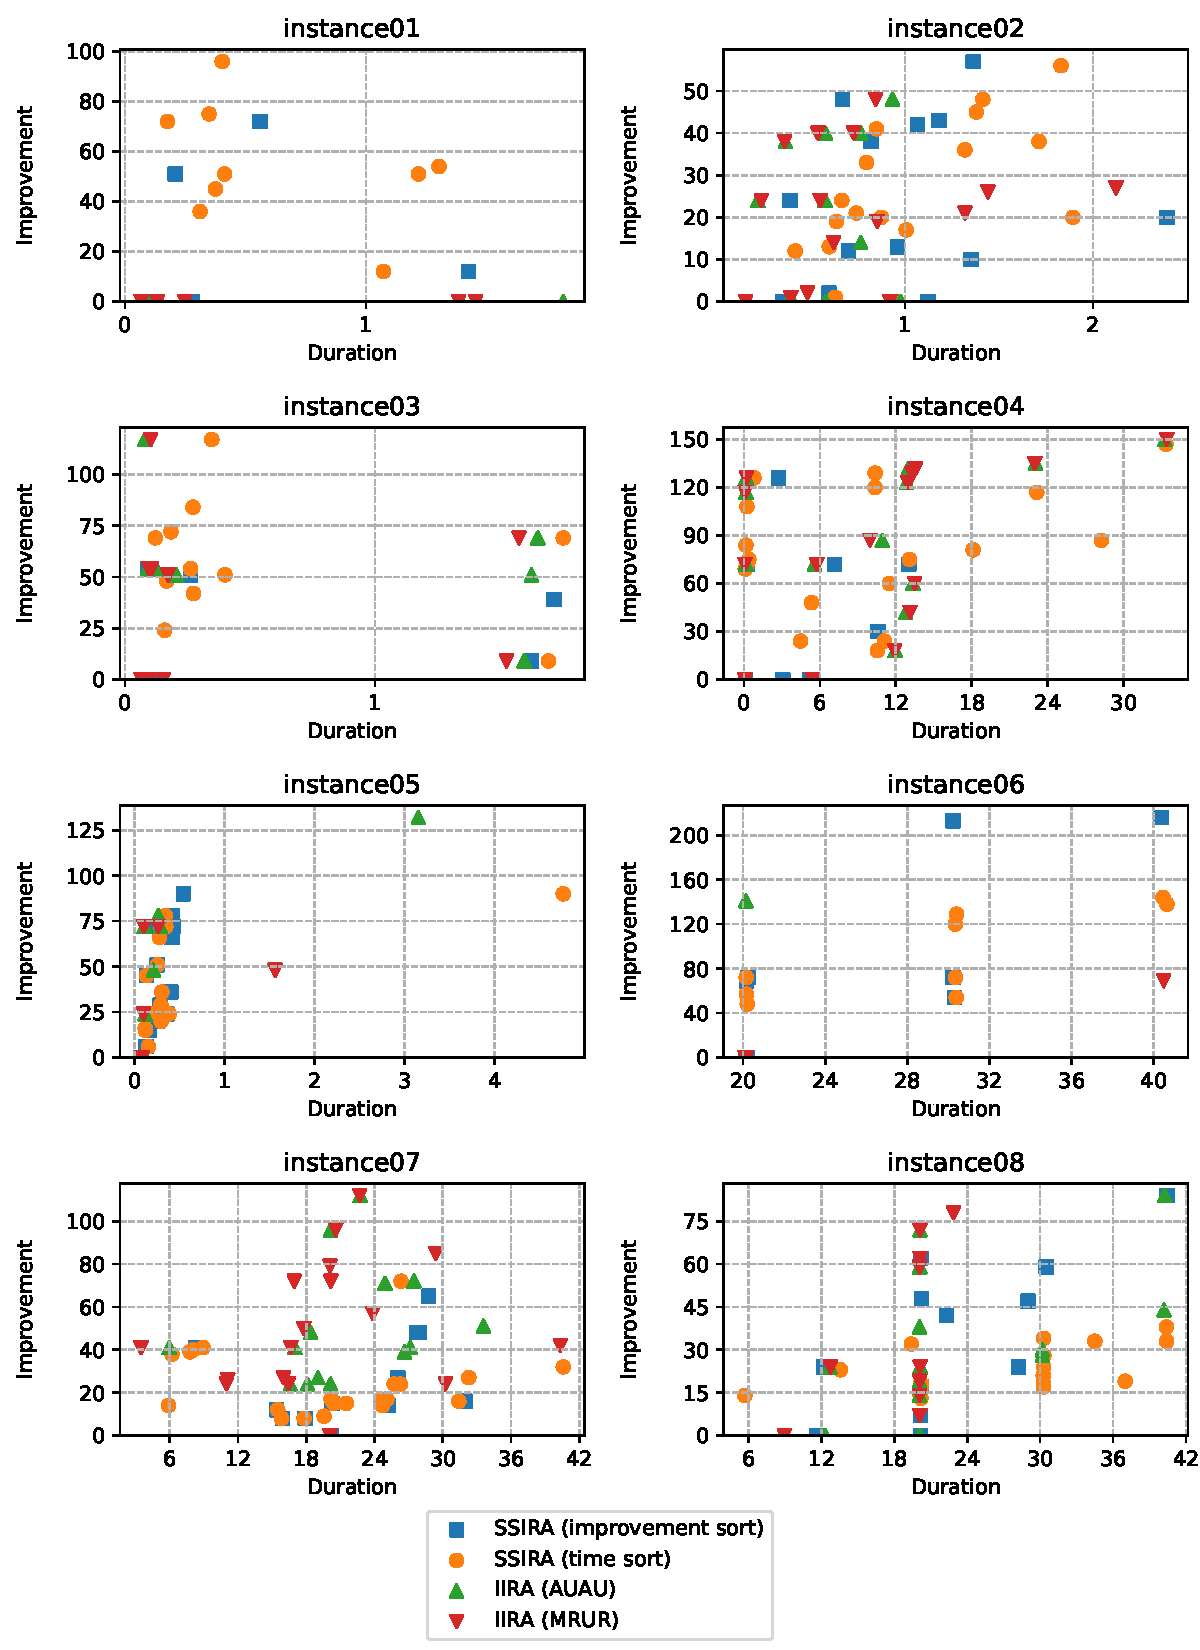
\includegraphics[width=\textwidth]{img/exp_aggregated_duration_improv.pdf}
    \caption{
        Aggregated plots of computation time (x-axis) to achieved improvement (y-axis).
        In each plot, every algorithm evaluation comprises of five Pareto fronts of evaluations
        on the five individual instances from the represented instance group.
        Full non-aggregated results for each individual instance can be found in \cref{fig:exp-full/duration-improv}.
        }
    \label{fig:exp/duration-improv}
\end{figure}

% ~~~~~~~~~~~~~~~~~~~~~~~~~~~~~~~~~~~~~~~~~~~~~~~~~~~~~~~~~~~~~~~~~~~~~~~~~~~~~~~~~~~~~~~~~~~~~~~~~~~~~~~~~~~
\section{Discussion} \label{sec:numerical-experiments/discussion}

The \ac{ssira} found improvements for all instances for which the \ac{iira} found improvements.
Furthermore, the \ac{ssira} found improvements for some instances where the \ac{iira} did not.
We can conclude that the \ac{ssira} has a higher probability of finding an improvement than the \ac{iira}.
We believe this is because, when seeking improvements, the \ac{iira} does not consider the target order.
Instead, it identifies bottleneck resources with respect to the whole problem instance
and its schedule.
Our theory is that this approach limits the \ac{iira} in cases
where the target order is not directly affected by execution bottlenecks
but is instead only partially constrained by the impact of the execution bottlenecks on the schedule.
In such cases, relaxations focused on the bottlenecks of the whole instance do not directly
improve the schedule with respect to the target order. 
This is where the \ac{ssira} benefits from its focused relaxations,
as all of its relaxations focus specifically on the target order.

As stated, the \ac{iira} does not consider the target order when finding improvements.
Nonetheless, it is able to find improvements at relatively low costs
compared to the solutions achieving the same improvements found by the \ac{ssira}.
Furthermore, on larger instances, the \ac{iira} finds solutions
with greater improvements and overall better quality than the \ac{ssira}.
This is an unexpected result,
as the initial assumption was that relaxations focusing specifically on the target order
would achieve better improvements than general relaxations.
We speculate that targeted relaxations of the \ac{ssira} might be too specific,
not providing sufficient slack in the modified constraints
and thus making the model too sensitive to minor variations when finding modified solutions.
Another possibility is that the \ac{ssira} often executes multiple relaxations simultaneously,
assuming their independence.
This assumption is inherent to the algorithm through the process it identifies potential relaxations.
When the presumed independent relaxations are implemented and the solver seeks a modified solution,
the combined relaxations might direct the solver towards a solution
that differs from what the algorithm intended.

Regarding the schedule difference induced by the proposed modifications,
the \ac{iira} is able to find better solutions that the \ac{ssira} on smaller instances.
On larger instances, the \ac{ssira} typically surpasses the \ac{iira} in performance.
This is likely because the \ac{iira} proposes general relaxations
whereas the \ac{ssira} proposes relaxations focusing on the target order.
On smaller instances, general relaxations usually affect most of the schedule,
but on larger instances, the impact of these relaxations becomes more local.
On larger instances, the systematic approach of the \ac{ssira} utilizing the focused relaxations
is able to find specific relaxations that are necessary to improve the target order.
Moreover, even on smaller instances, the \ac{ssira} is sometimes able to find solutions with
smaller impact on the schedule difference than the solutions of the \ac{iira}.
However, the general relaxing approach of the \ac{iira} is still viable on most instances.

We observed that on several instances,
distinct linear clusters of evaluations with identical evaluation times are formed.
In those clusters, the evaluations achieve varying improvements in the same amount of computation time.
Our theory is that the formation of those clusters is due to the set solver time limit,
which interrupts an evaluation if a solution has not been found in the specified time limit.
We can conclude that on such instances,
extending the solver time limit might result in better achieved improvements.
The introduction of the solver time limit represents a trade-off between solution quality and computation time,
particularly for more difficult instances.
Nonetheless, since the evaluations on most instances were not affected by the set time limit,
we conclude that the time limit was set appropriately in accordance with the difficulty of our problem.

We summarize the results in the following key points:
\begin{itemize}
    \item 
        The \ac{ssira} tends to find improvements more consistently than the \ac{iira},
        possibly because the \ac{ssira} proposes relaxations focused specifically on the target order,
        while the \ac{iira} proposes only general relaxations.

    \item
        Despite not directly considering the target order,
        the \ac{iira} tends to find improvements at lower costs
        and achieves solutions with greater improvements on larger instances compared to the \ac{ssira}.
        We theorize that this may be due to the \ac{ssira}'s specific relaxations being overly restrictive
        and that its execution of multiple relaxations simultaneously sometimes leads to unintended solutions.

    \item
        Regarding induced schedule difference,
        the \ac{iira} proposes better solutions on smaller instances,
        while the \ac{ssira} outperforms the \ac{iira} on larger instances.
        The \ac{ssira} sometimes achieves significantly better solutions than the \ac{iira}
        even on smaller instances, suggesting its viability across various problem sizes.
        However, the \ac{iira} proposes adequate solutions
        with acceptable solution differences more consistently.
\end{itemize}
